
\documentclass[journal]{IEEEtran}
\usepackage{blindtext}
\usepackage{graphicx}



% *** GRAPHICS RELATED PACKAGES ***
%
\ifCLASSINFOpdf
  % \usepackage[pdftex]{graphicx}
  % declare the path(s) where your graphic files are
  % \graphicspath{{../pdf/}{../jpeg/}}
  % and their extensions so you won't have to specify these with
  % every instance of \includegraphics
  % \DeclareGraphicsExtensions{.pdf,.jpeg,.png}
\else
  % or other class option (dvipsone, dvipdf, if not using dvips). graphicx
  % will default to the driver specified in the system graphics.cfg if no
  % driver is specified.
  % \usepackage[dvips]{graphicx}
  % declare the path(s) where your graphic files are
  % \graphicspath{{../eps/}}
  % and their extensions so you won't have to specify these with
  % every instance of \includegraphics
  % \DeclareGraphicsExtensions{.eps}
\fi






% correct bad hyphenation here
\hyphenation{op-tical net-works semi-conduc-tor}


\begin{document}
%
% paper title
% can use linebreaks \\ within to get better formatting as desired
\title{CSE 190: Predictive Policing on Crime Data}
\author{Joshua Wheeler,  Nathan Moreno, Anjali Kanak }

% make the title area
\maketitle

\begin{abstract}
In this report we discuss how data mining techniques can be used to solve predictive tasks related to crime data. We identify a set of predictive tasks, train and evalaute models to perform predictions and document the results.
\end{abstract}

\section{Introduction}
Predictive Policing is a modern solution to fundamental problems all police forces face today. Efficient allocation of resources and preemptive law enforcement. There are various predictive methods that help police departments determine when and where crime will happen before it happens. In this analysis, we will focus on two simple predictive tasks.
1) Predict whether or not an arrest will happen for a given incident
\\
2) Predict how many incidents of crime will happen in a beat on a given day. 

*Note: A beat is the geographical area a police officer is assigned to patrol. \\

The following sections describe the data set, findings from initial analysis, the prediction tasks identified and the results.  

\section{Dataset}

The dataset chosen for this assignment consists of incidents of crime reported in the city of Chicago from 2001 to 2015. The data set is approx. 5.8 million entries.  Each entry consists of the following fields:\\

\begin{center}
\begin{tabular}{| l | l |}\hline
Field & Description\\ \hline
sid & meta data\\ \hline
id & Record id \\ \hline
case\_number & Case number  \\ \hline
date & Date on which crime was reported \\ \hline
block & Block address of the crime \\ \hline
iucr & Code for the type of crime\\ \hline
primary\_type & Category of crime\\ \hline
description & Description of the crime \\ \hline
location\_description & short description of the location\\ \hline
arrest &  If arrest happened for the crime \\ \hline
domestic & If it was domestic violence \\ \hline
beat & Officers Patrol Area \\ \hline
district & District\\ \hline
ward & Ward \\ \hline
community\_area & Community area\\ \hline
fbi\_code & FBI code\\ \hline
latitude & Latitude \\ \hline
longitude & Longitude \\ \hline
year  &  Year in which the crime occurred\\ \hline
\end{tabular}
\end{center}

Some of the records had missing values for the fields and hence were excluded from training and test sets.

\section{Exploratory Analysis}
Data exploration helps infer useful information and predict important aspects of crime detection and prevention. At the same time, the nature of the data largely determines what kind of prediction tasks can be performed. A preliminary analysis of data was performed to identify useful features for building a predictive model. It revealed some interesting trends and patterns which are documented below.
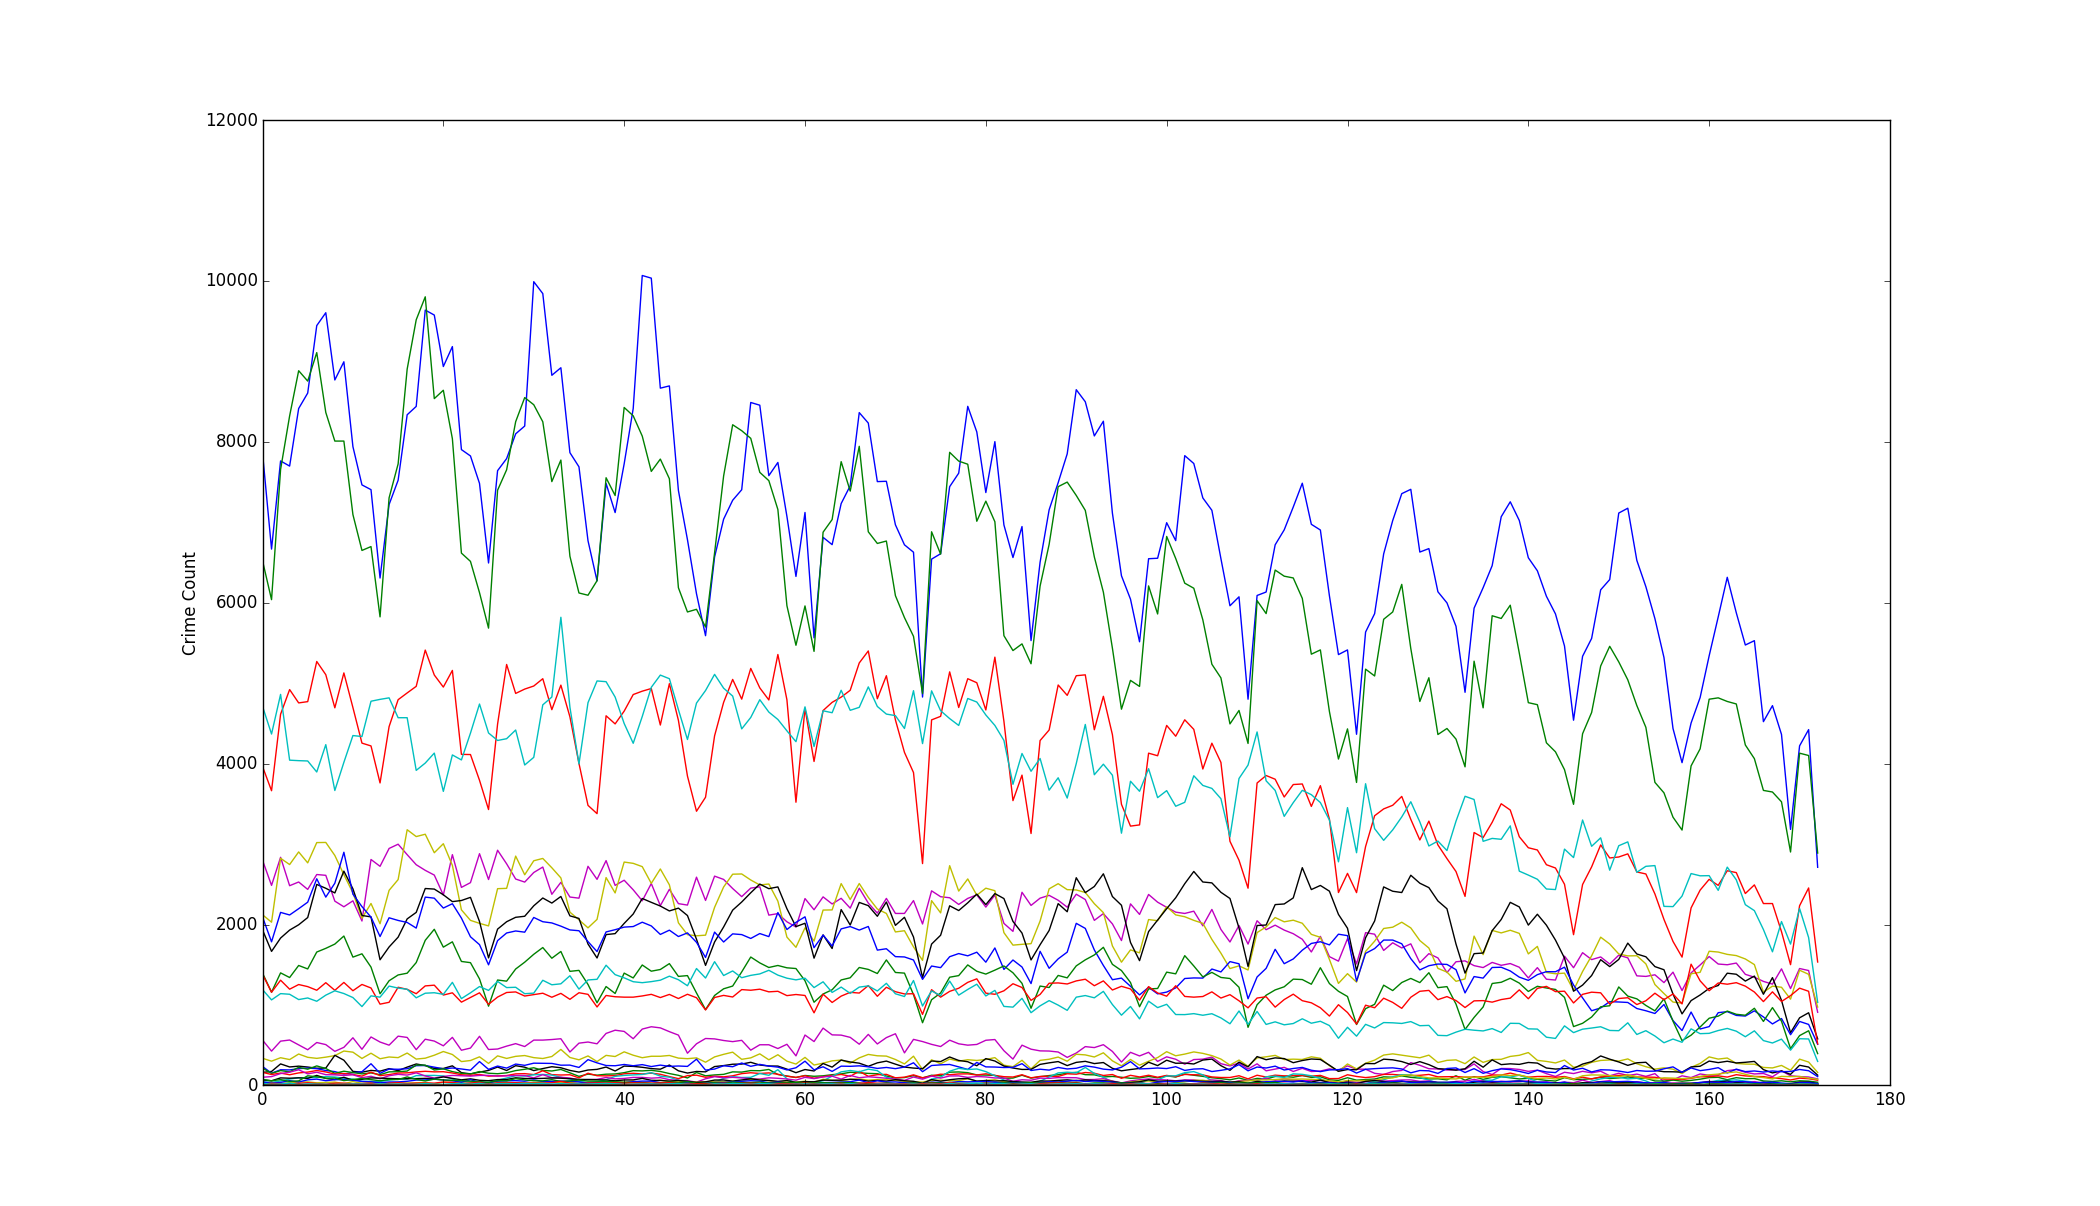
\includegraphics[scale = 0.17]{Crime/Month.png}

Figure 1: The above graph depicts crime rate for each category of crime over the span of 15 years. The crime rate is decreasing over years. Along this overall decrease, a periodic pattern can be observed every year where the crime rate is higher in summer compared to the rest of the year. 
Over the course of the year the incidents of crime for almost every category increases and decreases dramatically. We hypothesized this is the case for Chicago because it can get very cold. It seems crime increases as it gets warmer in the year and decreases as it gets colder throughout the year. This reasoning has not been verified, but it is known that the month of the year is directly correlated with crime rate. 

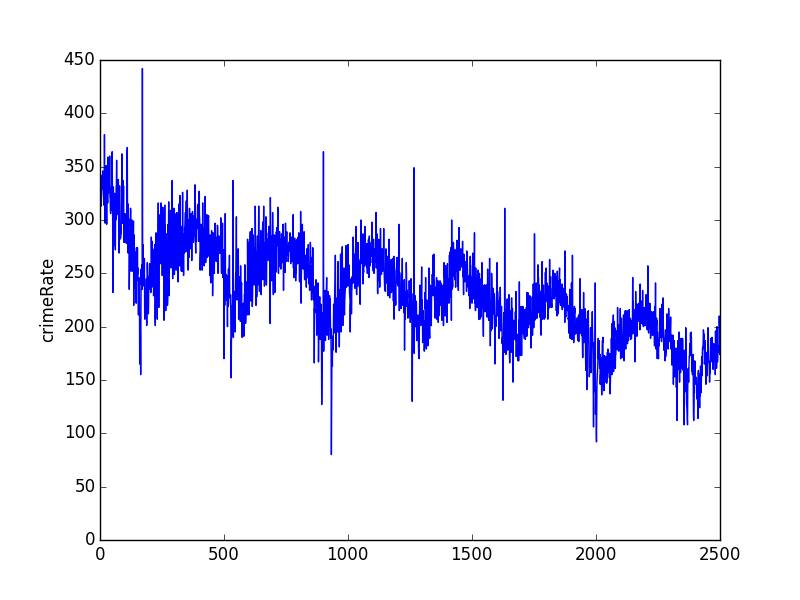
\includegraphics[scale = 0.27]{Crime/Day.jpg}

Figure 2:
This graph shows the rise and fall of all crime in Chicago with a resolution of a day over the span of 7 years. It reveals the same periodic, monotonically decreasing pattern as mentioned in Figure 1. 

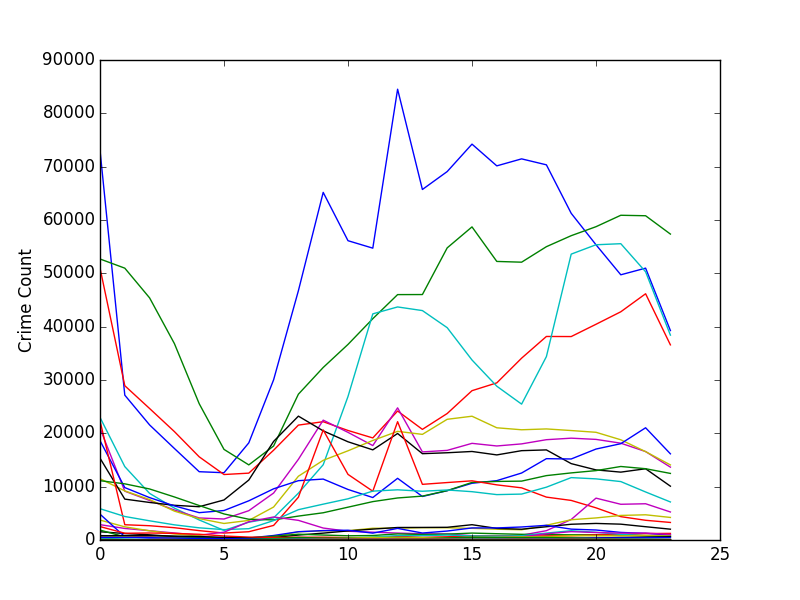
\includegraphics[scale = 0.4]{Crime/Hour.png}

Figure 3:
Shown by this graph, a cyclical pattern is consistently shown into the hours of the day. This data is the summation of all crime in the data set in a given hour for a type of crime. In this depiction, it can be observed that given the hour of the day, certain types of crime fall, while others rise. 
Furthermore, there seems to be a strong and consistent drop in crime early in the day; it might appear that crime does sleep, indeed - at approximately 05:00 AM in the morning.

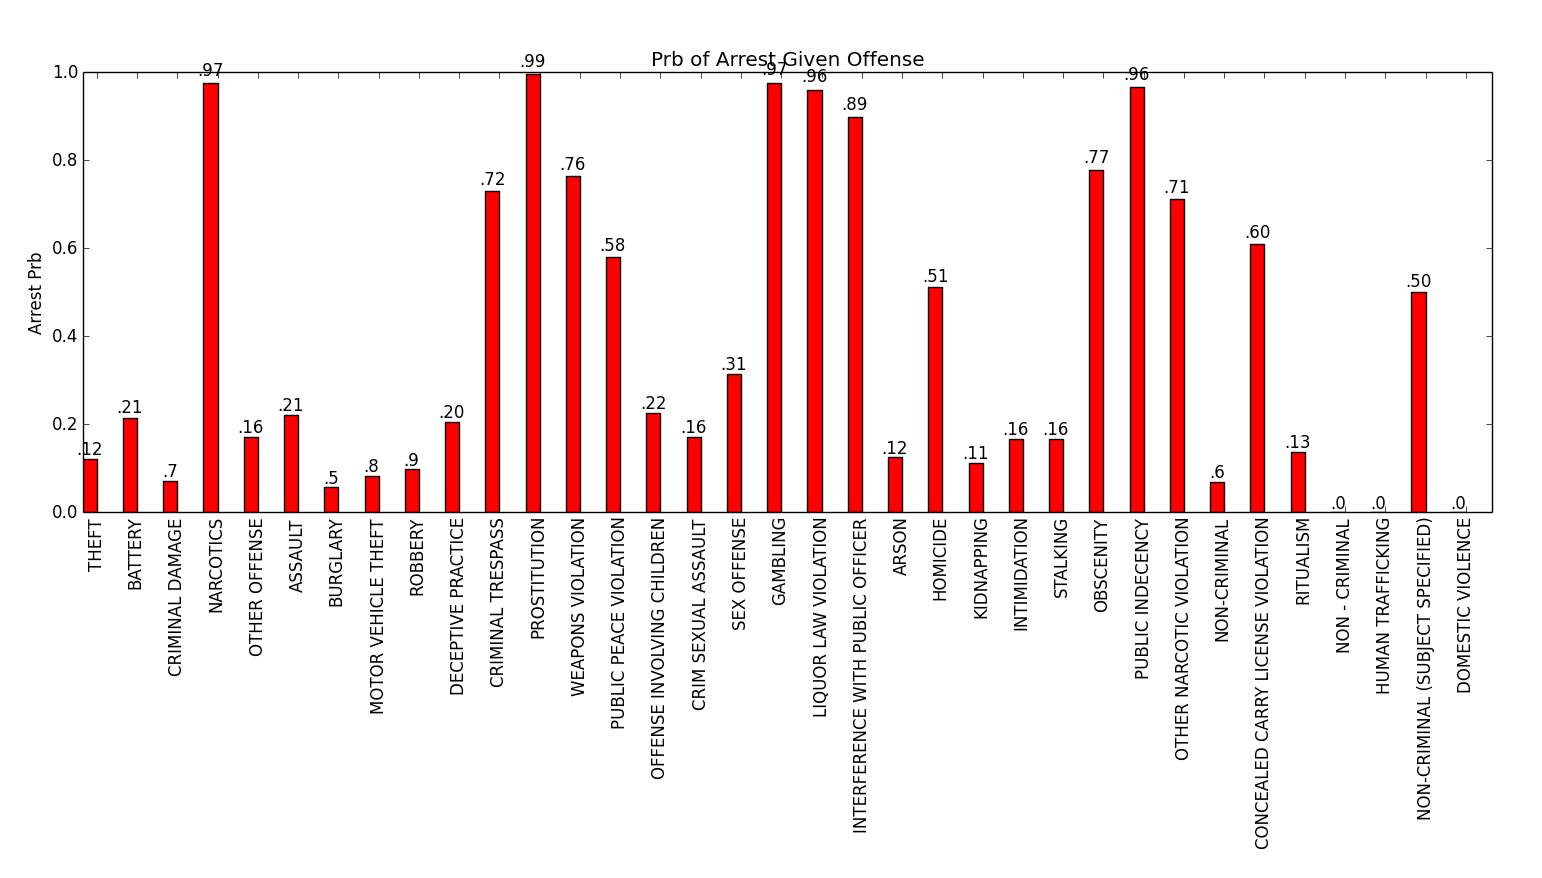
\includegraphics[scale = 0.15]{arrest1.jpg}
Figure 4:
The above Histogram reveals the probability of an arrest for a category of crime. 
It is shown that Narcotics offenses have the highest probability at around a 97 percent chance of a arrest given an offense. Others have lower probabilities of arrest such as Homicide with about a 50 percent chance of arrest. We think that the crimes that are easier to solve have a much higher probability of arrest than crimes that are harder to solve. The data is consistent with this hypothesis. 

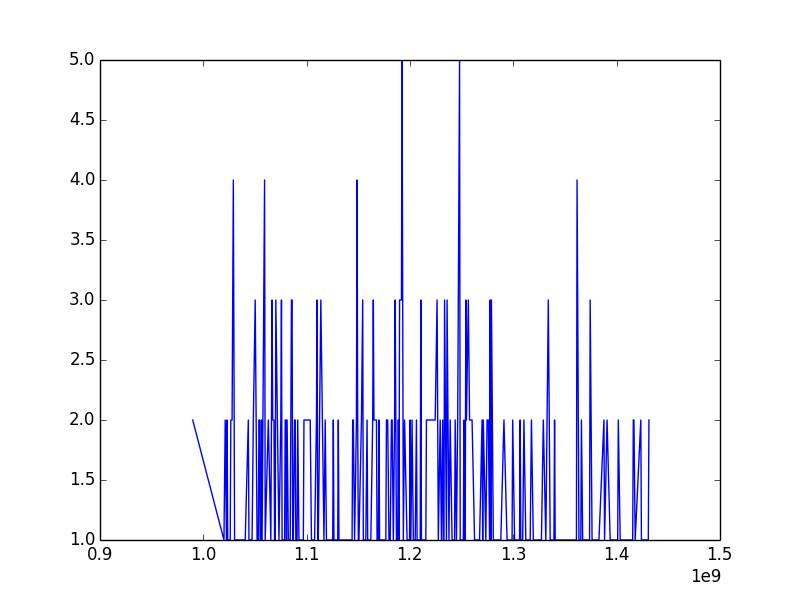
\includegraphics[scale = 0.3]{unknown.jpg}
Figure 5:
This graph shows the crime rate for consecutive city blocks. The Y axis represents the number of incidents of battery and the X axis is a given month. This data is graphed for a series of 11 city blocks. It can be seen that crime rate over time on the block level loses the periodic nature that is revealed in the prior graphs.


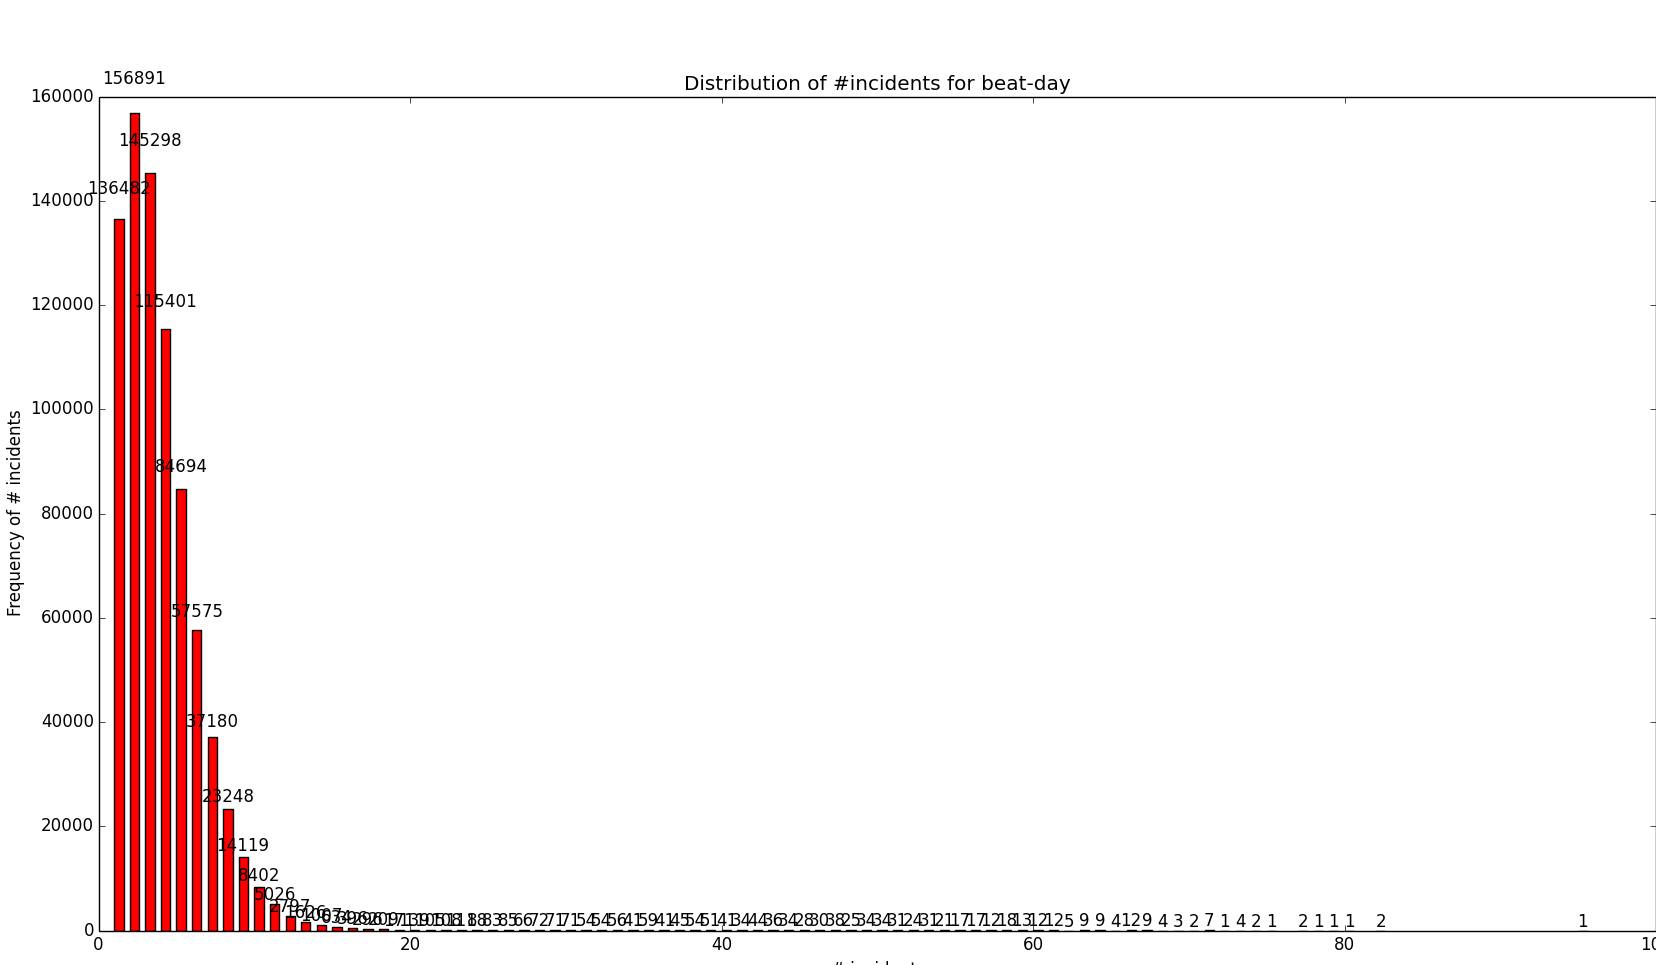
\includegraphics[scale = 0.14]{incidents.jpg}
Figure 6:
This histogram is a graph of the frequency of an incident number for a beat-day. 
Using this information it is possible to extract statements like "It is most common for 2 crimes to happen in a police beat in a given day" or "It is second most common for 1 crime to happen in a police beat on a given day". These insights help to understand the distribution of incident frequencies for a police beat in a day. 


\section{Predictive Task}

We identified two predictive tasks based on the information available in the data set. 

\subsection{\textbf{Predicting whether an arrest will be made for a committed crime}}
Our first predictive task was to predict arrests for reported crimes.
A prediction can be shown in the following format - \\
CASE NUMBER: \hspace{1cm} ARREST\\
HM776500 \hspace{2cm}	0\\
where the first column is the case number and the second column is whether or not an arrest will be made for this case number. 

To perform this prediction we used logistic regression. This model was chosen as opposed to other models such as naive bayes' because our analysis indicated to us that the positive and negative correlations in the trends in our features would have greater accuracy than using the counting nature of conditional probabilities. We also decided to use this over SVM's to save computation time. 

\begin{enumerate}
\item 
We used a baseline to predict the arrest likelihood based on past arrests before applying our model. For the baseline, we first calculate the probability of an arrest as a ratio of number of arrests to the number incidents of a given crime type. On the test data, a crime is predicted to result in an arrest if the arrest probability for the respective type of crime is greater than 0.5 and is predicated as no arrest otherwise.\\ This baseline is similar to a naive bayes calculation. 

\item Logistic Regression
 The feature vector was chosen based on the pre-processing done during the exploratory analysis. Three features were considered:
\begin{enumerate}
\item Month in  which the crime happened represented as a 12 feature vector
\item Type of crime such as Narcotics, Battery etc. represented as a 34 feature vector, one for each crime type.  This was represented as a feature vector with categorical labels (1 if present, 0 if absent).  A total of 32 categories were identified.
\item Location description: A short description of the street/location in which the crime happened.  The location description was used as a categorical label and represented as a binary value (1 if the feature was present, 0 if absent).
\end{enumerate}

Month was chosen because our exploratory analysis indicates that it is a seasonal influence in crime rate. This is revealed in Figure 1. Since it is correlated with the rate of crime, by transitivity it is also correlated with the arrest rate for the crime. If there is more crime in a month then correspondingly, there will be more arrests. 

Our analysis also indicated that the probability of an arrest is heavily influenced by crime type. Figure 4 reveals that there are high disparities in arrest rate with some of the crime categories. Since this is the case, it seems that crime type is a strong predictor of whether or not there will be an arrest. 

The location description was thought to influence arrest rate as well because it seems that it is more common for arrests to be made in some locations more often than others. For example, it may be more likely for an individual to be arrested for battery in the middle of a parking lot than in a more discrete location such as an alley way. This feature was added because of this qualitative assumption. We found that the score improved after adding this as a feature.

All of the features were represented as binary vectors in order to allow equal representation and individual weights for each possible choice of each feature. Pre-processing was done on all of the categorical variables in order to map them to their corresponding binary feature vector representations. 

For assessing validity of this classification, the Hamming Loss is used where the total score is calculated as 
            $$1-HammingLoss(x_i,y_i)= 1 - \frac{1}{|D|}\sum \frac{xor(xi,yi)}{|L|}$$
For this application, this can be interpreted as the percentage of correct predictions as to whether or not there was an arrest for the crime.
\end{enumerate}

\subsection{\textbf{Predicting how many crimes will happen in a police beat over the time period of a given day}}
The second predictive task used was to predict how many crimes are likely to happen in a police beat in a given day. 
A prediction is represented in the following format:\\
DATE: \hspace{1cm}	BEAT: \hspace{1cm} NUM\_INCIDENTS: \\
2002-09-18 \hspace{0.5cm}	 1631 \hspace{1cm}	 3

Where we are trying to predict the NUM\_INCIDENTS column given the date and beat identifier. 

Two models were considered as a solution to this problem. The first model in consideration which was not chosen was a latent factor model where a bias for the month and bias for the beat would be calculated. We decided that this model would not be effective because there were not enough date-beat pairs to calculate a solid bias on. 
Instead, we decided to use a Linear Regression to approach this problem. In this problem we noticed that features do exist that are both positively and negatively correlated with the number of incidents for a beat-day pair. 

\begin{enumerate}
\item 
The Baseline: Figure 6 in the exploratory analysis indicated that one to two crimes were amongst the most popular for a beat-day pair. From this observation, a constant beat-day baseline was chosen. NUM\_INCIDENTS in this baseline is predicted to always be 1. The results section later in this document reveal that this is a decent prediction when the data set is medium sized but becomes weaker as the data set becomes very large. 

\item Our Model: In order to develop a more accurate predictor, a logistic regression was used. Two categorical features were chosen and pre-processed as n-length feature vectors where n is the number of possible categories for the feature. The features chosen are as follows
\begin{enumerate}
\item Month - The month is represented as a 12 dimension feature vector. The vector is all zero's except for the feature with the current month of the day being evaluated. This month is given a value of 5 in the vector. 
\item Crime Type - The crime type is represented as a 34 dimension feature vector. This vector is all zeros except for all of the types of crimes that happened for the given beat-day pair. In this vector, multiple elements can be on. If a crime type is on in this feature vector it is given a representative value of 10. 
\end{enumerate}

Month was chosen for this model for the same reason as the first arrest prediction task. Crime frequency has a seasonal aspect to it. The main difference between this vector and that of task one is that if a month is "on" in this vector, it is given a representative value of 5. This is because the prediction for NUM\_INCIDENTS needs to be boosted for more accuracy. 

The crime type was chosen for this model because analysis showed that incidents of some crimes are more frequent than others. People deal drugs much more often than they commit homicides for example. The fact that some crimes happened during a beat-day and another did not influences how many crimes may have happened during a given beat-day. 

Other features such as block number were not used because they were too noisy as shown by Figure 5. 

In order to score this model the Absolute Error was used. Mathematically absolute error is defined as 
    $$ AE = \sum |\hat{y_i} - y_i| $$
With regard to this application absolute error is interpreted as the total number of incidents that were incorrectly predicted.
\end{enumerate}

\section{Literature Survey}

Different research groups and organizations have analysed different aspects of crime detection. What can be predicted and which data mining technique can be employed to do the prediction depends on the information available directly or indirectly from the data set.  Some of the research papers[1] focused on clustering techniques to detect co-relation between different types of crimes, identifying groups of offenders etc.  Information about the convict and the victim are necessary to identify patterns in crime. The data set we used does not include information about the criminal or the victim.\\ 

Specific to data analytic techniques for crime detection we looked at papers and books related to this area. Upon searching for literature already discussing predictive methods for law enforcement, we found a book on predictive policing with descriptions of various models used for predictive analytics pertaining to crime analysis. We have been using this information as inspiration to design our own models used in this report.[2]

\section{Evaluation and Results}
The following section documents the evaluation results for the predictive tasks described in the previous section. Baselines are defined and predictive models are built in an attempt to improve the baseline performance.  The  results are documented and analysed. 

For each predictive task, we split the data set into training and test set. We then trained the models and used them to predict the labels on the test set.

\subsection{Predicting whether an arrest will be made for a crime}
The table below compares the results from the baseline prediction and the model based on logistic regression for a training data set of size 100K entries and a test data set of size 50K entries.

\begin{center}
\begin{tabular}{| l | l | l | l | l | l |}\hline
Model & TP & TN & FP & FN & Accuracy\\ \hline
Baseline & 7464 & 36283 & 770 & 5483 & 0.87492\\ \hline
Log. Reg. & 7998 & 35966 & 1087 & 4949 & 0.87926\\ \hline
\end{tabular}
\end{center}

Logistic regression performs better than the baseline in predicting the true negatives, true positives and false negatives.  The number of false positive is  higher than the baseline.  However, this does not have a serious impact and hence is acceptable.

The accuracy is comparable in both cases, but unfortunately the model did not outperform the baseline prediction on the given data set. This indicates that the arrest probability for the type of crime committed has a very strong influence in whether or not there will be an arrest. Adding additional features to the predictor was negligible and did not yield better results.

\subsection{Prediction score for the number of crimes in a beat\-day}
Small Dataset: (200K training, 50K test)
\begin{center}
\begin{tabular}{| l | l | l |}\hline
Model & Num incidents & Absolute Error\\ \hline
Baseline & 50000 & 10892\\ \hline
Model & 50000 & 5440\\ \hline
\end{tabular}
\end{center}

When trained on a moderate amount of data, the model substantially outperformed the baseline with approx 200 percent improvement on absolute error. This indicates that month and crime type do have predictive power in determining the amount of crime for a beat-day. At this scale of data the model is 89\% accurate. Note that accuracy is calculated in the following way: 
$$ 1 - (\frac{absolute\_error}{num\_incidents}) $$


Large Dataset (3M training, 2M test):
\begin{center}
\begin{tabular}{| l | l | l |}\hline
Model & Num incidents & Absolute Error\\ \hline
Baseline & 2000000 & 1571518\\ \hline
Model & 2000000 & 486975\\ \hline
\end{tabular}
\end{center}

If the model is trained on a large amount of data, the baselines is still substantially out performed with approx 300\% improvement on absolute error but the accuracy declines as the data size grows. 
At this scale, the model is 75\% accurate, this is a drop of roughly 14\% from the medium sized set. This decrease in accuracy may either be due to natural variation or the fact that as data scales the distribution of num\_incident frequencies increases and thus becomes harder to predict.

\section{Conclusion}
In this project, we used data mining techniques to perform predictive tasks on crime data. Two predictive tasks were implemented - predicting arrests for a given type of crime in a given location and predicting number of crimes in a police beat on a given day. Pre-processing of data prior to training the model helped us identify useful features for building the models. The models used the techniques we learnt in the course. The results from evaluation are discussed and documented.  

Though we observed repeated patterns in crime count over months with summer being the highest, it did not add value to the prediction of whether or not arrests will be made but did help influence the prediction for number of crimes in a beat-day. The type of crime also played strong role in predicting arrests and crime frequencies in Chicago.

These tasks can be further extended to include much more extensive patterns in predictive crime if information about the victims and the offenders are made available. 

\section{References}
[1] Learning to Detect Patterns of Crime Tong Wang1, Cynthia Rudin, Daniel Wagner and Rich Sevier, Massachusetts Institute of Technology, Cambridge, MA 02139, USA

[2] Perry, Walter L., Brian McInnis, Carter C. Price, Susan Smith and John S. Hollywood. Predictive Policing: The Role of Crime Forecasting in Law Enforcement Operations. Santa Monica, CA: RAND Corporation, 2013.  $http:\/\/www.rand.org/pubs/research_reports/RR233$.

[3] Crime Pattern detection using data mining, Shyam Varan Nath, Oracle Corporation

[4] The data set used for this project: https://data.cityofchicago.org/Public-Safety/Crimes-2001-to-present/ijzp-q8t2

\end{document}


